\documentclass[8pt]{beamer}
% Add references to notes
\makeatletter\defbeameroption{show only notes}[]{\beamer@notestrue\beamer@notesnormalsfalse}

% Originally from https://kbroman.org/blog/2013/10/07/better-looking-latexbeamer-slides/
\usetheme{default}
\hypersetup{pdfpagemode=UseNone} % hides bookmarks on initial view
\beamertemplatenavigationsymbolsempty % removes navigation buttons clashing with the defined slide numbers

\setbeamertemplate{sections/subsections in toc}[sections numbered] % replaces bullets in toc with numbers
\setbeamertemplate{bibliography item}{\insertbiblabel} % Numbered bibliography
\setbeamertemplate{itemize subitem}{{\textendash}} % changes bullets to \textendash
% Make bullets/nums smaller
\setbeamerfont{itemize/enumerate subbody}{size=\footnotesize}
\setbeamerfont{itemize/enumerate subitem}{size=\footnotesize}
% Slide number
 \setbeamertemplate{footline}{%
   \raisebox{5pt}{\makebox[\paperwidth]{\hfill\makebox[20pt]{\color{gray}
         \scriptsize\insertframenumber}}}\hspace*{5pt}}

\definecolor{foreground}{RGB}{255,255,255}
\definecolor{background}{RGB}{24,24,24}
\definecolor{title}{RGB}{107,174,214}
\definecolor{gray}{RGB}{155,155,155}
\definecolor{subtitle}{RGB}{102,255,204}
\definecolor{hilight}{RGB}{102,255,204}
\definecolor{vhilight}{RGB}{255,111,207}

\setbeamercolor{titlelike}{fg=title}
\setbeamercolor{subtitle}{fg=subtitle}
\setbeamercolor{institute}{fg=gray}
\setbeamercolor{normal text}{fg=foreground,bg=background}
\setbeamercolor{item}{fg=foreground} % color of bullets
\setbeamercolor{subitem}{fg=gray}
\setbeamercolor{itemize/enumerate subbody}{fg=gray}
\setbeamercolor{section in toc}{fg=foreground}
\setbeamercolor{subsection in toc}{fg=gray}


\usepackage{amsmath} % for more symbols and mafs
\usepackage{hyperref} % for links
\usepackage{fancyvrb}
\usepackage{hyperref}

\usepackage{array}
\newcolumntype{M}{>{\centering\arraybackslash}m{2.2cm}}
\newcolumntype{R}{>{\centering\arraybackslash}m{1.5cm}}

\usepackage{caption}
\captionsetup{justification=raggedleft} % right aligns multiline captions

\graphicspath{{../images/}}

\usepackage[backend=biber, sorting=none]{biblatex}
\addbibresource{../bib.bib}

\usepackage{xepersian} % must be the last package
\settextfont{XB Roya}
\setlatintextfont{Vazir}
\setdigitfont{XB Roya}
\setmonofont{Iosevka}
\usefonttheme{serif} % (Required for Persian)

\makeatletter
% Originally from http://qa.parsilatex.com/14100
% -----
% BEGIN List fix
% -----
\expandafter\let\csname beamer@@tmpop@itemize item@default\endcsname\relax
\expandafter\let\csname beamer@@tmpop@itemize subitem@default\endcsname\relax
\expandafter\let\csname beamer@@tmpop@itemize subsubitem@default\endcsname\relax

\defbeamertemplate*{itemize item}{default}{\scriptsize\raise1.25pt\hbox{\donotcoloroutermaths$\blacktriangleleft$}}
\defbeamertemplate*{itemize subitem}{default}{\tiny\raise1.5pt\hbox{\donotcoloroutermaths$\blacktriangleleft$}}
\defbeamertemplate*{itemize subsubitem}{default}{\tiny\raise1.5pt\hbox{\donotcoloroutermaths$\blacktriangleleft$}}

\patchcmd{\@listi}{\leftmargin}{\rightmargin}{}{}
\let\@listI\@listi
\patchcmd{\@listii}{\leftmargin}{\rightmargin}{}{}
\patchcmd{\@listiii}{\leftmargin}{\rightmargin}{}{}
\patchcmd{\beamer@enum@}{\raggedright}{\raggedleft}{}{}
\patchcmd{\@@description}{\raggedright}{\raggedleft}{}{}
\patchcmd{\@@description}{\leftmargin}{\rightmargin}{}{}

\renewcommand{\itemize}[1][]{
  \beamer@ifempty{#1}{}{\def\beamer@defaultospec{#1}}
  \ifnum \@itemdepth >2\relax\@toodeep\else
    \advance\@itemdepth\@ne
    \beamer@computepref\@itemdepth% sets \beameritemnestingprefix
    \usebeamerfont{itemize/enumerate \beameritemnestingprefix body}%
    \usebeamercolor[fg]{itemize/enumerate \beameritemnestingprefix body}%
    \usebeamertemplate{itemize/enumerate \beameritemnestingprefix body begin}%
    \list{\usebeamertemplate{itemize \beameritemnestingprefix item}}{\def\makelabel##1{{
      \hss\llap{{
        \usebeamerfont*{itemize \beameritemnestingprefix item}
        \usebeamercolor[fg]{itemize \beameritemnestingprefix item}##1}}
      }}
    }
  \fi
  \beamer@cramped
  \raggedleft
  \beamer@firstlineitemizeunskip
}
% -----
% END List fix
% -----
% BEGIN TOC fix
% -----
\expandafter\let\csname beamer@@tmpop@subsection in toc@default\endcsname\relax
\expandafter\let\csname beamer@@tmpop@subsubsection in toc@default\endcsname\relax
\defbeamertemplate*{subsection in toc}{default}
{\leavevmode\rightskip=1.5em\inserttocsubsection\par}

\defbeamertemplate*{subsubsection in toc}{default}
{\leavevmode\normalsize\usebeamerfont{subsection in toc}\rightskip=3em
  \usebeamerfont{subsubsection in toc}\inserttocsubsubsection\par}
% -----
% END TOC fix
% -----
\makeatother

\raggedleft % right aligns for Persian texts


\author{محمدیاسین داوده}
\title{لینوکس}
\subtitle{هرآنچه لازم است بدانید}
\date{\today}

\newcommand{\start}[1][نقشه راه]{
  \frame{\maketitle}
  \begin{frame}{#1}\tableofcontents\end{frame}
}

\newcommand{\bib}{
  \begin{LTR}
    \printbibliography[heading=none]
  \end{LTR}
}

\newcommand{\refs}{
  \section{مراجع}
  \begin{frame}[allowframebreaks]{مراجع}
    \bib
  \end{frame}
  \note{\bib}
}

\newcommand{\subt}[1]{{\footnotesize\color{subtitle}{#1}}}

\newcommand{\divider}[1]{\frame{\Huge{#1}}}

\newcommand{\subdivider}[1]{\frame{\color{hilight}\huge{#1}}}

\newcommand{\alongside}{\and\\\small\smallskip}

\newcommand{\singleton}[2][]{
  \begin{frame}{#1}
    \centering
    #2
  \end{frame}
}

\newcommand{\includetwins}[3][\textwidth]{
  \includegraphics[width=.49#1]{#2}
  \includegraphics[width=.49#1]{#3}
}
% -----
% BEGIN Code (minted)
% -----
\newenvironment{code*}[2][]{
  \VerbatimEnvironment
  \begin{LTR}
    \begin{minted}[#1, linenos, mathescape]{#2}%
    }{
    \end{minted}
  \end{LTR}
}

\newcommand{\codecaption}[1][]{\captionsetup{type=listings}\captionof{listing}{#1}}

\AtBeginEnvironment{minted}{\renewcommand{\fcolorbox}[4][]{#4}} % Disable syntax error red boxes
% -----
% END Code (minted)
% -----


\begin{document}
\start

% فارسی
\begin{frame}{سیستم عامل}
  \begin{figure}
    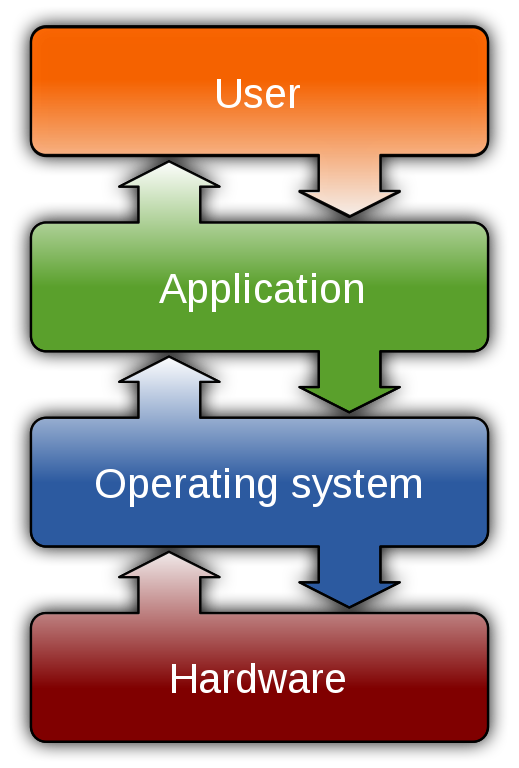
\includegraphics[width=.4\textheight]{os}
    \caption*{سیستم عامل رابط بین کاربر و سخت‌افزار~\cite{fig:wp:os}}
  \end{figure}
\end{frame}
\note{سیستم‌عامل خوب مثل دوربین خوب در یک بازیست. بهترین سیستم‌عامل آنی است که متوجه وجود آن نشوید. وظیفهٔ آن ارائه رابط و منابع به برنامه‌ها است. از دو بخش کرنل (رابط بین ابزارها و هسته سیستم) و ابزارهای مرتبط و سیستمی ساخته می‌شود.}
\section{تاریخچه}
\begin{frame}{یونیکس}
  \begin{figure}
    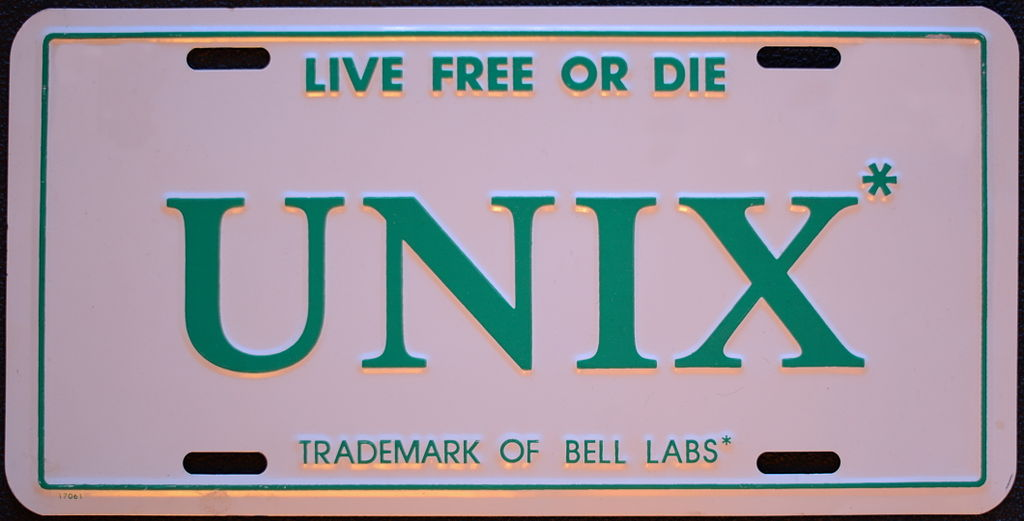
\includegraphics[width=.8\textwidth]{unix_plate}
    \caption*{سیستم عامل نوین یونیکس بر پایه C~\cite{fig:wp:unix_plate}}
  \end{figure}
\end{frame}
\note{
  ساختهٔ ۱۹۷۰ آزمایشگاه بل توسط \lr{Ken Thompson}, \lr{Dennis Ritche} و چندی دیگر.

  سیستم‌عامل خصوصی غالب دهه ۷۰. هزینه‌بر و کندتر از سیستم‌عامل‌های دورهٔ خودش.

  در آن دوره سیستم‌عامل‌ها با نرم‌افزارهای خاص خودشان و بعضاً با سخت‌افزارهای خودشان منتشر می‌شدند.
}
\begin{frame}{ریچارد متیو استالمن (R.M.S)}
  \begin{figure}
    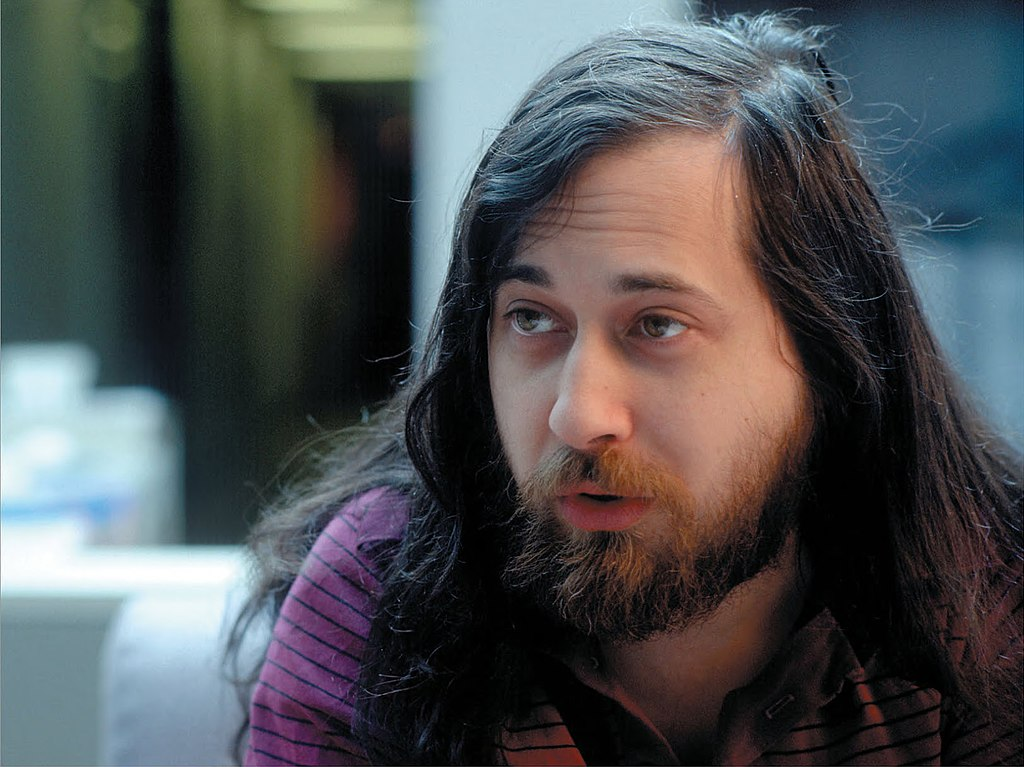
\includegraphics[width=.8\textheight]{rms}
  \caption*{
    عکس ریچارد متیو استالمن بنیانگذار \textit{بنیاد نرم‌افزارهای آزاد (FSF)
      % \LTRfootnote{Free Software Foundation}
    } و \textit{پروژهٔ گنو} بر جلد \textit{آزاد مانند آزادی: جهاد ریچارد استالمن برای نرم‌افزار آزاد
      % \LTRfootnote{Free as in Freedom: Richard Stallman's Crusade for Free Software}
    } نوشتهٔ \textit{سم ویلیامز
      % \LTRfootnote{Sam Williams}
    }~\cite{fig:wp:rms}
  }
  \end{figure}
\end{frame}
\note{
  تا زمانی که مایکروسافت مفهوم نسبتاً جدید «نرم‌افزار خصوصی (\lr{Proprietory})» را در اواخر دهه ۷۰ مطرح کرد. نرم‌افزار تقریباً آزادانه قابل انتقال و اشتراک‌گذاری بود.

  استالمن سال ۷۱ وارد آزمایشگاه هوش مصنوعی MIT شد که به علت محدودیت‌های یونیکس سیستم‌عامل خود را ساخته بودند. نام آن سیستم اشتراک زمانی ناسازگار (Incompatible Timesharing System) بود. (ریچارد استالمن)

  اریک ریموند (مؤلف «کلیسا و بازار») نقل می‌کند که استالمن تجارب بدی با نرم‌افزارهای خصوصی آزمایشگاه MIT داشت (می‌خواست نرم‌افزارهایی که خریده بود را ویرایش کند اما شرکت اجازه حل مشکل را به او نمی‌داد).
  استالمن بر این باور بود که نگه داشتن کد و اشتراک نگذاشتن آن به مثل تک-خوری در دانش و توسعه است.

  استالمن بر آن شد تا بنیادی در خلاف این حقوق دست‌وپاگیر بنا کند و سیستم‌عاملی آزاد از این حقوق بنویسد. بنابراین بنیاد نرم‌افزارهای آزاد بنا شد.

  در ژانویه ۸۴ استفا داد و شروع به توسعه پروژه گنو کرد: GNU is Not Unix

 ابتدا به تنهایی و بعداً با کمک جامعه، یکی یکی تمام ابزارهای یونیکس را بازنویسی کرده و در انتها در صدد بازنویسی کرنل بودند.
  \cite{ros}
}
\begin{frame}[fragile]{آزاد مثل آزادی}
  \vfill
  \begin{figure}
    \begin{LTR}
      \centering
      \Huge
      \begin{BVerbatim}
Free Software
    Free Society
      \end{BVerbatim}
    \end{LTR}
    \vfill
    \caption*{آزادی نرم‌افزار حرکتی اجتماعی است.}
  \end{figure}
\end{frame}
\note{
  آزادی به معنی وجود توانایی تغییر است. نه به معنی رایگان.
  یعنی بتوانید نرم‌افزار خود را تغییر دهید، منتشر کنید و دیگران از نسخه بهتر استفاده کنند.

  آزادی فرصت همکاری و جامعه شدن را می‌دهد. در صورت نبود این آزادی شرکت‌ها سلطه بر دارایی‌ها خواهند داشت.
}
\begin{frame}{مجوزهای آزاد}
\begin{table}
  \resizebox{\textwidth}{!}{%
  \begin{tabular}{R||M|M|M|M|M|M}
    & \multicolumn{3}{c}{آزاد و باز (نرم‌افزار باید سورس کد را نیز شامل شود)} & \multicolumn{3}{c}{غیرآزاد}\\\hline
    & مالکیت عمومی و مثل آن & مجوز آسانگیر & کپی لفت (محافظتی) & غیرتجاری & خصوصی & اسرار تجاری\\\hline\hline
    توضیحات &
              شامل تمام حقوق &
              اجازه استفاده و باز مجوزدهی را می‌دهد (شامل خصوصی‌سازی) &
              حقوق استفاده را می‌دهد و خصوصی‌سازی را منع می‌کند. &
              فقط اجازهٔ استفادهٔ غیرتجاری و اشتراک با مجوز مشابه را می‌دهد. &
              کپی رایت سنتی؛ نیاز نیست هیچ حقی ارائه کند. &
              هیچ اطلاعاتی عمومی نشود.\\\hline
    مجوزهای نرم‌افزاری & \lr{PD, CC0} & \lr{BSD, MIT, Apache, MPL} & \lr{{\color{hilight}GPL, AGPL}} & \lr{JRL, AFPL} & خصوصی؛ بدون مجوز عمومی & نرم‌افزار داخلی\\\hline
    مجوز دیگر کارهای خلاقانه & \lr{PD, CC0} & \lr{CC-BY} & \lr{CC-BY-SA} & \lr{CC-BY-NC} & کپی‌رایت؛ بدون مجوز عمومی & منتشر نشده
  \end{tabular}}
  \caption*{مقایسه چند مجوز عام~\cite{wp:copyleft}}
\end{table}
\end{frame}
\note{
  مجوزهای (License) عمومی کپی رایت برای نرم‌افزارهای آزاد هم موجودند و عمومی نیستند در نتیجه شما نمی‌تواند اعلام کنید مالک اثری آزادی هستید مگر اینکه مجوز آنرا داشته باشید.

  مجوزهای کپی‌رایت نشان می‌دهند که چه کسی می‌تواند اثری را منتشر کند و صاحب معنوی آن است.

  در صورت نبودن مجوز نمی‌توانید ادعای مالکیت روی اثری را کنید. از نگرانی‌های استالمن استفاده از نرم‌افزارهای آزاد و برنامه‌های نوشته شده در محصولاتی است که آزاد نیستند و از دست رفتن نام نویسنده اصلی در این میان بود.

  تمام مجوزهای آزاد کپی‌لفت نیستند و اجباری به نگه‌داری آزادی در آنها نیستند مانند مجوزهای BSD و MIT.
}
\begin{frame}{متن‌باز؟ متن-باز؟ آزاد یا رایگان؟}
  \begin{itemize}
    \item متن باز می‌تواند چند معنی داشته باشد.
    \begin{itemize}
      \item متن-باز تعریفی دارد که در \href{https://opensource.org/osd}{Opensource.org/osd} به صراحت بیان شده است.
      \item متن باز به صرف دیدن متن واقعاً نرم‌افزاری را متن-باز نمی‌کند.
    \end{itemize}
    \item آزادی تعریفی دارد که در بنیاد نرم‌افزارهای آزاد بیان شده است.
    \item آزاد هیچگاه لزوماً به معنی متن-باز، و هیچگاه لزوماً به معنی رایگان نمی‌باشد.~\cite{freevsos}
  \end{itemize}
\end{frame}
\note{
  آزادی‌های لازم برای \textit{آزاد} قلمداد شدن یک نرم‌افزار~\cite{freedef}:
  \begin{enumerate}
    \setcounter{enumi}{-1}
    \item آزادی اجرای نرم‌افزار در صورت اراده کردن و به هر دلیلی.
    \item آزادی مطالعه نحوهٔ کار برنامه، و تغییر آن جهت وادار آن به محاسبه به نحوی که می‌خواهید. (دسترسی به سورس کد برنامه یک پیشنیاز این مورد است.)
    \item آزادی بازنشر آن جهت کمک به دیگران.
    \item آزادی نشر نسخه‌های ویرایش‌شده به دیگران. (با انجام این کار این فرصت پیش می‌آید تا کل جامعه از تغییرات شما استفاده کنند.)(دسترسی به سورس کد برنامه یک پیشنیاز این مورد است.)
  \end{enumerate}
}\note{
  شرایط متن-باز بودن برنامه‌ها~\cite{osd}:
  \begin{enumerate}
    \item بازنشر رایگان (شامل رسانهٔ حامل نرم‌افزار نمی‌شود.)
    \item سورس کد قابل دسترسی و رایگان (معمولاً همراه بسته) که قابل بازنشر باشد. فرم کامپایل شده هم باید شامل این شرایط باشد.
    \item باید اجازهٔ ویرایش و بازنشر ویرایشات و کارهای مشتق‌شده را حتی تحت مجوز کار اصلی بدهد.
    \item مجوز باید اجازهٔ بازنشر بیلدهای حاصله از کدهای ویرایش شده را حتی به تحت نامی دیگر بدهد.
    \item در مجوز آن تبعیضی علیه اشخاص یا گروهی خاص نباشد.
    \item در مجوز آن تبعیضی علیه حوزه‌های مختلف کاری نباشد.
    \item حقوق الحاقی به برنامه باید به گونه‌ای که نیازی به انجام هیچ کار اضافی توسط آن اشخاص نباشد، شامل تمام افرادی که برنامه به آنها بازنشر می‌شود باشد.
    \item مجوز نباید محدود به محصولی خاص باشد. مجوز نباید وابسته به نرم‌افزاری دیگر باشد یا تأکید به همراهی نرم‌افزار در توزیعی خاص داشته باشد.
    \item مجوز نباید نرم‌افزارهای دیگر را محدود کند.
    \item مجوز باید بی‌تفاوت و بی‌طرف به نصب فناوری باشد. مجوز نباید دلالت بر فناوری یا رابطی خاصی کند.
  \end{enumerate}
}
\begin{frame}{لینوس توروالدز}
  \begin{figure}
    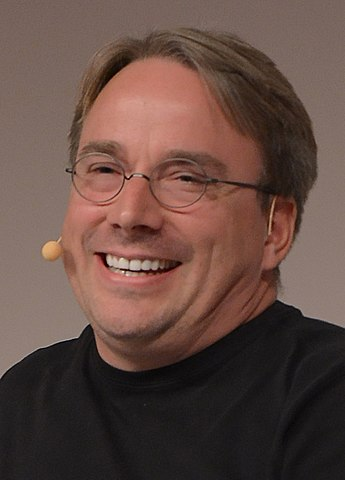
\includegraphics[width=.4\textheight]{linus}
    \caption*{لینوس توروالدز خالق \textit{لینوکس: سیستم‌عامل قابل حمل}~\cite{fig:wp:linus}}
  \end{figure}
\end{frame}
\note{
  جدا از پروژهٔ گنو که تا اوایل دههٔ ۹۰ تقریباً کامل بود و فقط هستهٔ آن در حال توسعه بود~\cite{ros}، لینوس توروالدز با الهام از سیستم‌عامل \textit{مینیکس} (یونیکس کوچک)
  \textit{اندرو تننباوم} (مستند در کتاب \textit{سیستم‌های عامل: طراحی و پیاده‌سازی}) تز ارشد خود را \textit{لینوکس: سیستم‌عامل قابل حمل} نام نهاد.
  نسخهٔ اولیهٔ سیستم‌عامل او در سال ۱۹۹۱ و نسخهٔ یکم آن در ۱۴ مارچ ۹۴ تحت مجوز GPL منتشر شد.~\cite{wp:linus}
}

\refs
\end{document}
